\documentclass[twoside,openany]{book}
\usepackage{amsmath}
\usepackage{geometry}
\usepackage{setspace}
\usepackage{titlesec}
\usepackage{booktabs}
\usepackage{caption}
\usepackage{tabularx}
\usepackage{array}
\usepackage{ragged2e}
\usepackage{tikz}
\usetikzlibrary{calc}
\usetikzlibrary{positioning}

\geometry{bindingoffset=0.5in, left=1.25in, right=1.25in, top=1.25in, bottom=1.25in}
\onehalfspacing
\raggedbottom
\titleformat{\chapter}[display]
    {\normalfont\huge\bfseries}{}{0pt}{\Huge}
\setlength{\parindent}{15pt}
\setlength{\parskip}{0pt} 
\sloppy                     

\begin{document}

\chapter*{Last-minute additions after the consultation}

\section*{Prerequisites: Keynesian, IS-LM, and AD-AS Frameworks}
A solid understanding of the following models is essential. 

\subsection*{Comparison of Macroeconomic Frameworks}

\begin{table}[ht]
    \centering
    \small
    \begin{tabularx}{\textwidth}{|X|X|X|X|}
    \hline
    \textbf{Model} & \textbf{Price and Wage Flexibility} & \textbf{Core Mechanism} & \textbf{Policy Implications} \\
    \hline
    Keynesian Cross & Fixed prices and wages & Demand determines output; government spending has a direct effect & Fiscal policy is highly effective; monetary policy not considered \\
    \hline
    IS-LM Model & Fixed prices in short run & Interaction of goods (IS) and money (LM) markets determines interest rates and output & Both fiscal and monetary policies matter; crowding-out effect can occur \\
    \hline
    AD-AS Model & Short-run price stickiness; long-run flexibility & Aggregate demand and supply interaction determines output and prices & Long-run effects depend on supply-side factors; both demand and supply policies matter \\
    \hline
    \end{tabularx}
    \caption{Comparison of Keynesian, IS-LM, and AD-AS Models}
\end{table}

\newpage

The formulas below are provided for reference of what are the factors affecting slopes, not some actual formulas which should be consulted while solving tasks.

\textbf{Keynesian Cross:}
\begin{align*}
    Y &= C + I + G \\
    C &= C_0 + c(Y - T) \\
    \text{Multiplier} &= \frac{1}{1 - c (1 - t) + m}
\end{align*}

\textbf{IS-LM Model:}
\begin{align*}
    \text{IS: } & Y = C(Y - T) + I(r) + G \\
    \text{LM: } & \frac{M}{P} = L(Y, r)
\end{align*}

\textbf{AD-AS Model:}
\begin{align*}
    \text{AD: } & Y = f(P, \text{demand}) \\
    \text{SRAS: } & Y = f(W, \text{costs}) \\
    \text{LRAS: } & Y = Y^*
\end{align*}

\section*{Money and Banking Multipliers}
\begin{itemize}
    \item \textbf{Money Multiplier:} When the \emph{required reserve ratio} falls, the money multiplier increases. This expansion in the multiplier effect enlarges the monetary base, subsequently shifting the Aggregate Demand (AD) curve to the right.
    \item \textbf{Banking Multiplier:} Similarly, the ability of banks to create loans (the banking multiplier) is enhanced when reserve requirements are relaxed, further contributing to an increase in the money supply.
\end{itemize}

\section*{Interactions among IS, LM, and AD Curves}
\begin{itemize}
    \item The AD curve is closely linked to the IS-LM framework. A rightward shift in the IS curve—indicating increased equilibrium output—typically results in a corresponding rightward shift in AD.
    \item \textbf{Expansionary Policies:} Stimulative measures, such as fiscal or monetary expansion, shift the IS, LM, and AD curves to the right, reinforcing aggregate demand across multiple channels.
\end{itemize}

\section*{Supply-Side Adjustments}
\begin{itemize}
    \item \textbf{Short-Run Aggregate Supply (SRAS):} The SRAS curve is primarily influenced by changes in the labor market. For example, shifts in wage dynamics directly affect production costs and, consequently, the supply side of the economy.
    \item If nominal wages increase—and if real wages rise accordingly—production costs go up. Firms may then hire fewer workers, leading to a leftward shift in the SRAS curve.
\end{itemize}

\section*{Marginal Propensity to Consume (MPC) and Its Impact on AD}
\begin{itemize}
    \item An increase in the \emph{marginal propensity to consume} (MPC) raises overall consumption (C), which is a major component of aggregate demand.
    \item In general, any factor that boosts consumption or investment will shift the AD curve to the right.
\end{itemize}
\chapter*{Essential Formulas}

\subsection*{Macroeconomic GDP Formulas}
\begin{itemize}
    \item Expenditure Approach:
    \[ GDP = C + I + G + (X - Z) \]
    \item Income Approach:
    \[ GDP = \text{Labor Income} + \text{Capital Income} \]
    \item Output (Value Added) Approach:
    \[ GDP = \sum \text{Value Added} \]
    \item Savings-Investment Identity:
    \[ Y = C + S \quad \text{and} \quad Y = C + I \quad \Rightarrow \quad S = I \]
    \item Nominal GDP:
    \[ \text{Nominal GDP} = \sum (\text{Quantity} \times \text{Current Price}) \]
    \item Real GDP:
    \[ \text{Real GDP} = \sum (\text{Quantity} \times \text{Constant Price}) \]
    \item GDP Deflator:
    \[ \text{GDP Deflator} = \frac{\text{Nominal GDP}}{\text{Real GDP}} \times 100 \]
\end{itemize}

\subsection*{Keynesian Cross Model Formulas}
\begin{itemize}
    \item \textbf{Consumption Function (No Government):}
    \[
    C = A + cY
    \]
    where \(A\) is autonomous consumption and \(c\) (with \(0<c<1\)) is the marginal propensity to consume.
    \item \textbf{Investment (Exogenous):}
    \[
    I = \bar{I}
    \]
    \item \textbf{Aggregate Demand (AD):}
    \[
    AD = A + cY + \bar{I}
    \]
    \item \textbf{Equilibrium Output (No Government):}
    \[
    Y^* = \frac{A + \bar{I}}{1 - c}
    \]
    Here, \(\frac{1}{1-c}\) is the multiplier.
    \item \textbf{Consumption Function (With Government):}
    \[
    C = A + c(1-t)Y
    \]
    where \(t\) is the net tax rate.
    \item \textbf{Equilibrium Output (With Government):}
    \[
    Y^* = \frac{A + \bar{I} + G}{1 - c(1-t)}
    \]
    \item \textbf{Savings-Investment Identity:}
    \[
    S = Y - C = I
    \]
    \item \textbf{Balanced Budget Multiplier:} Conceptually, a \$1 increase in government spending financed by an equal increase in taxes leads to an increase in equilibrium output by \$1.
\end{itemize}

\subsection*{Additional Macroeconomic Formulas (Lecture II.3)}
\begin{itemize}
    \item \textbf{Open Economy Equilibrium (with Government):}
    \[
    Y^* = \frac{A + \bar{I} + G + \bar{X}}{1 - c(1-t) + z}
    \]
    where \(z\) is the marginal propensity to import.
    \item \textbf{Real Interest Rate (Inflation-Adjusted):}
    \[
    r_{\text{real}} \approx r_{\text{nominal}} - \pi
    \]
    with \(\pi\) being the inflation rate.
    \item \textbf{Debt-to-GDP Ratio:}
    \[
    \text{Debt-to-GDP Ratio} = \frac{\text{Government Debt}}{Y}
    \]
    \item \textbf{Money Multiplier:}
    \[
    mm = \frac{1 + cr}{cr + rr + er}
    \]
    where \(cr\) is the currency-deposit ratio, \(rr\) the required reserve ratio, and \(er\) the excess reserve ratio.
    \item \textbf{Deposit Multiplier:}
    \[
    \text{Deposit Multiplier} = \frac{1}{rr}
    \]
    \item \textbf{Loan Multiplier:}
    \[
    \text{Loan Multiplier} = \frac{1 - rr}{rr}
    \]
    \item \textbf{Money Market Equilibrium:}
    \[
    M_d(Y, r) = M_s
    \]
    and real money balances are given by \(\frac{M}{P}\).
    \item \textbf{Definitions of Money Aggregates:}
    \[
    M0 = \text{Currency outside banks}
    \]
    \[
    MB = M0 + \text{Reserves held by banks}
    \]
    \[
    M1 = C + D \quad (\text{with } C=\text{currency},\, D=\text{demand deposits})
    \]
\end{itemize}

\subsection*{IS-MP Model Formulas (Lecture II.4)}
\begin{itemize}
    \item \textbf{Investment Function:}
    \[
    I = I_0 + \text{mpi} \cdot Y - b \cdot i
    \]
    where \(I_0 > 0\) is autonomous investment, \(\text{mpi} \in (0,1)\) is the marginal propensity to invest, and \(b > 0\) captures investment’s sensitivity to the interest rate.
    \item \textbf{Consumption Function:}
    \[
    C = A_0 - a \cdot i + c(1-t) \cdot Y
    \]
    where \(A_0 > 0\) is autonomous consumption, \(a > 0\) is the sensitivity of consumption to the interest rate, \(c \in (0,1)\) is the marginal propensity to consume, and \(t\) is the net tax rate.
    \item \textbf{Goods Market Equilibrium:}
    \[
    Y = C + I + G + NX
    \]
    with \(NX\) representing net exports.
    \item \textbf{Derived IS Curve:}
    \[
    Y\Bigl(1 - c(1-t) - \text{mpi} + z\Bigr) = \Bigl[A_0 + I_0 + G + X\Bigr] - (a+b)i
    \]
    where \(z\) is the marginal propensity to import.
    \item \textbf{Equilibrium Output (IS Relation):}
    \[
    Y^* = \frac{A_0 + I_0 + G + X - (a+b)i}{1 - c(1-t) - \text{mpi} + z}
    \]
    \item \textbf{Monetary Policy Assumption:} Under fixed prices (GDP deflator \(=1\)), nominal and real interest rates are identical.
\end{itemize}

\subsection*{AD-AS Model and Taylor Rule (Lecture II.5)}
\begin{itemize}
    \item \textbf{Aggregate Demand (AD):}
    \[
    AD = C + I + G + (X - Z)
    \]
    (Note: In this model, AD is influenced by monetary policy through its effect on consumption and investment.)
    \item \textbf{Short-Run Aggregate Supply (SRAS):}
    Due to sticky wages, the SRAS is upward sloping. Firms determine output based on the real wage:
    \[
    MPL = \frac{w}{p}
    \]
    where \(MPL\) is the marginal product of labor, \(w\) the nominal wage, and \(p\) the price level.
    \item \textbf{Long-Run Aggregate Supply (LRAS):}
    With flexible wages and prices, the economy operates at potential output:
    \[
    Y = Y^*
    \]
    \item \textbf{The Taylor Rule:}
    The rule for setting the nominal interest rate is given by:
    \[
    r - r^* = a(\pi - \pi^*) + b(Y - Y^*)
    \]
    or, for nominal rates,
    \[
    i - i^* = (1+a)(\pi - \pi^*) + b(Y - Y^*)
    \]
    where \(a>0\) and \(b>0\) measure the responsiveness to inflation and the output gap.
\end{itemize}
\chapter*{Keynesian Cross Model}

The Keynesian Cross Model is a simple framework to analyze the equilibrium in the goods and services market. In this model, actual output \(Y\) is determined by planned expenditure. In a closed economy with no government, the equilibrium condition is given by:
\[
Y = C + I,
\]
where
\[
C = A + cY \quad \text{and} \quad I = \bar{I}.
\]
Thus, aggregate (or planned) expenditure (AD) becomes
\[
AD = A + cY + \bar{I}.
\]
Equilibrium occurs when \(Y = AD\), so that:
\[
Y = A + cY + \bar{I} \quad \Longrightarrow \quad Y^* = \frac{A + \bar{I}}{1 - c}.
\]
Here, \(\frac{1}{1-c}\) is the multiplier, which shows how a change in autonomous spending leads to a magnified change in equilibrium output.

An alternative expression involves the saving function. Since
\[
S = Y - C = Y - (A + cY) = -A + (1-c)Y,
\]
the equilibrium condition \(S = I\) reinforces that any change in autonomous spending \(A\) (or \(\bar{I}\)) affects \(Y\) by a factor of \(\frac{1}{1-c}\).

\bigskip

\textbf{Key Formulas for the Keynesian Cross Model:}
\begin{itemize}
    \item Consumption Function (no government):
    \[
    C = A + cY
    \]
    \item Investment (exogenous):
    \[
    I = \bar{I}
    \]
    \item Aggregate Demand:
    \[
    AD = A + cY + \bar{I}
    \]
    \item Equilibrium Output:
    \[
    Y^* = \frac{A + \bar{I}}{1 - c}
    \]
    \item Saving Function:
    \[
    S = Y - C = -A + (1-c)Y
    \]
    \item \textbf{Multiplier:} \(\dfrac{1}{1-c}\)
\end{itemize}

\bigskip

\textbf{Diagram of the Keynesian Cross Model}

Below is a typical diagram for the Keynesian Cross. In this diagram, the 45° line (blue) represents the points where actual output \(Y\) equals planned expenditure. The planned expenditure line (red) is given by:
\[
\text{Planned Spending} = A + \bar{I} + cY.
\]
Equilibrium occurs where the planned spending line intersects the 45° line.

For example, assume:
\[
A + \bar{I} = 5 \quad \text{and} \quad c = 0.6.
\]
Then the planned spending line is:
\[
PS(Y) = 5 + 0.6Y.
\]
Equilibrium is determined by:
\[
Y = 5 + 0.6Y \quad \Longrightarrow \quad 0.4Y = 5 \quad \Longrightarrow \quad Y^* = 12.5.
\]

\begin{tikzpicture}[scale=0.3]
    \draw[->] (0,0) -- (20,0) node[right] {\(Y\)};
    \draw[->] (0,0) -- (0,20) node[above] {Planned Spending, AD};
    \draw[thick,blue] (0,0) -- (20,20);
    \draw[thick,red] (0,5) -- (20,17);
    \fill (12.5,12.5) circle (7pt);
    \node[xshift=-0.7cm, yshift=0.25cm] at (12.5,12.5) {\(Y^*=12.5\)};
  \end{tikzpicture}

\textbf{Interpretation:}
\begin{itemize}
    \item The diagram shows that when autonomous spending (i.e., \(A+\bar{I}\)) increases, the planned spending line shifts upward, leading to a higher equilibrium output.
    \item Conversely, an increase in the marginal propensity to consume \(c\) amplifies the multiplier effect, meaning that any change in autonomous spending produces a larger change in output.
    \item The \emph{Paradox of Thrift} is illustrated by the saving function: if households decide to save more (i.e., a decrease in \(A\)), equilibrium output falls by a multiple of that change, leaving total saving \(S\) unchanged if investment \(I\) remains exogenous.
\end{itemize}

\bigskip

\textbf{Additional Discussion:}
This model is foundational in macroeconomics. Although it makes simplifying assumptions—such as exogenous investment and no government—the Keynesian Cross provides essential insights into the multiplier effect and the dynamics of output determination. As the model is extended to include government and an open economy, the basic principles remain, though the formulas become more complex (e.g., incorporating taxes and imports).
\chapter*{The IS--LM Model}
\section*{1. Standard IS-LM Framework (Upward-Sloping LM Curve)}
\begin{figure}[h!]
    \centering
    \begin{tikzpicture}[scale=1.0]
        \draw[->] (0,0) -- (5.5,0) node[right] {$Y$ (Output)};
        \draw[->] (0,0) -- (0,5.5) node[above] {$i$ (Interest Rate)};
        \draw[thick,blue] (1,4) -- (4,1) node[right] {IS};
        \draw[thick,red] (1,1) -- (4,4) node[right] {LM};
        \draw[dotted] (2.5,0) -- (2.5,2.5) -- (0,2.5);
        \draw (2.5,2.5) node[circle,fill,inner sep=1.5pt]{};
        \node[yshift=0.33cm] at (2.5,2.5) {$E$};
    \end{tikzpicture}
    \caption{A simple IS-LM diagram with an upward-sloping LM curve. 
    The intersection at $E$ represents the equilibrium in both the goods and money markets.}
\end{figure}

\noindent
\textbf{Interpretation:} 
\begin{itemize}
    \item \emph{IS line (blue)}: Shows the inverse relationship between the interest rate $i$ and output $Y$ that equilibrates the goods market (higher $i$ reduces investment and thus reduces $Y$).
    \item \emph{LM line (red)}: Reflects the positive relationship between $Y$ and $i$ in the money market (more output raises money demand, pushing up the interest rate).
    \item \emph{Equilibrium ($E$)}: Where the two lines intersect, determining the simultaneous equilibrium in both markets.
\end{itemize}

\section*{2. IS--LM Model with a Fixed Interest Rate (Horizontal LM)}
\begin{figure}[h!]
    \centering
    \begin{tikzpicture}[scale=1.0]
        \draw[->] (0,0) -- (5.5,0) node[right] {$Y$ (Output)};
        \draw[->] (0,0) -- (0,5.5) node[above] {$i$ (Interest Rate)};
        \draw[thick,blue] (1,4) -- (4,1) node[right] {IS};
        \draw[thick,red] (0.5,2.5) -- (5,2.5) node[right] {LM ($i$ fixed)};
        \draw[dotted] (2.5,0) -- (2.5,2.5) -- (0,2.5);
        \draw (2.5,2.5) node[circle,fill,inner sep=1.5pt]{};
        \node[above right] at (2.5,2.5) {$E'$};
    \end{tikzpicture}
    \caption{IS-LM diagram with a fixed interest rate. The LM curve is horizontal, 
    indicating that the central bank keeps $i$ constant regardless of output $Y$.}
\end{figure}

\noindent
\textbf{Interpretation:}
\begin{itemize}
    \item With a fixed interest rate, the LM curve becomes perfectly elastic (horizontal). 
    \item Any change in $Y$ does not affect $i$, as the central bank accommodates changes in money demand by adjusting the money supply.
    \item The new equilibrium $E'$ remains at the same interest rate but can shift in terms of output if the IS line moves (e.g., due to fiscal policy).
\end{itemize}

\section*{IS Curve Shift: Decrease in Autonomous Investment}
A decrease in autonomous investment (\(\bar{I}\)) reduces aggregate demand for any given interest rate, causing the IS curve to shift left (i.e., equilibrium output is lower at every interest rate). The magnitude of this shift depends on the relevant multiplier:
\[
\text{Multiplier} = 
\begin{cases}
\frac{1}{1-c} & \text{(Closed economy, no government)},\\[1em]
\frac{1}{1 - c(1-t)} & \text{(Closed economy, with government)},\\[1em]
\frac{1}{1 - c(1-t) + z} & \text{(Open economy, with imports)}.
\end{cases}
\]
Here, \(c\) is the marginal propensity to consume, \(t\) the net tax rate, and \(z\) the marginal propensity to import. A drop in \(\bar{I}\) therefore shifts the IS curve left by \(\Delta \bar{I}\) times the relevant multiplier.
\begin{figure}[h!]
    \centering
    \begin{tikzpicture}[scale=1.0]
        \draw[->] (0,0) -- (5.5,0) node[right] {$Y$ (Output)};
        \draw[->] (0,0) -- (0,5.5) node[above] {$i$ (Interest Rate)};
        \draw[thick,blue] (1,4) -- (4,1) node[right] {$\text{IS}_1$};
        \draw[thick,purple] (1,3) -- (3,1) node[right] {$\text{IS}_2$};
        \draw[thick,red] (1,1) -- (4,4) node[right] {LM};
        \draw[dotted] (2.5,0) -- (2.5,2.5) -- (0,2.5);
        \draw (2.5,2.5) node[circle,fill,inner sep=1.5pt]{};
        \node[yshift=0.33cm] at (2.5,2.5) {$E_1$};
        \draw[dotted] (2,0) -- (2,2) -- (0,2);
        \draw (2,2) node[circle,fill,inner sep=1.5pt]{};
        \node[yshift=0.33cm] at (2,2) {$E_2$};
    \end{tikzpicture}
    \caption{Leftward shift of the IS curve (\(\text{IS}_1 \to \text{IS}_2\)) due to a decrease in autonomous investment. 
    Equilibrium moves from \(E_1\) to \(E_2\), reducing both output (\(Y\)) and the interest rate (\(i\)) in this example.}
\end{figure}

\noindent
\textbf{Key Points:}
\begin{itemize}
    \item \textbf{Autonomous Investment Decreases:} For a given interest rate, firms reduce their planned investment, lowering aggregate demand.
    \item \textbf{IS Curve Shifts Left:} Equilibrium output is smaller at every interest rate.
    \item \textbf{Multiplier Effect:} The total change in output depends on how large the multiplier is, which in turn depends on the structure of the economy (presence of taxes, openness to trade, etc.).
    \item \textbf{New Equilibrium:} The economy moves from \(E_1\) to \(E_2\), where output \(Y\) is lower and, in this example, the interest rate \(i\) is also somewhat lower.
\end{itemize}

\section*{Factors Causing a Leftward Shift of the IS Curve}
\noindent
The IS curve represents equilibrium in the goods market: 
\[
Y = C + I + G + NX.
\]
A leftward shift means that, at any given interest rate $i$, the equilibrium level of output $Y$ is lower. This can result from:
\begin{itemize}
    \item \textbf{Decrease in Autonomous Consumption:}
    \begin{itemize}
        \item Households reduce their consumption due to lower consumer confidence, a negative wealth effect (e.g., a decline in stock or housing prices), or pessimistic future income expectations.
        \item This lowers aggregate demand directly.
    \end{itemize}
    \item \textbf{Decrease in Autonomous Investment:}
    \begin{itemize}
        \item Firms reduce planned investment (e.g., due to lower business confidence, less optimistic profit expectations, or stricter lending standards).
        \item This reduces aggregate demand and shifts the IS curve left.
    \end{itemize}
    \item \textbf{Decrease in Government Spending ($G$):}
    \begin{itemize}
        \item If the government cuts its expenditures (for instance, due to austerity measures or attempts to reduce budget deficits), then for any given interest rate, total planned spending is lower.
        \item The IS curve shifts left by the change in $G$ multiplied by the relevant fiscal multiplier.
    \end{itemize}
    \item \textbf{Increase in Taxes ($T$) or Net Tax Rate ($t$):}
    \begin{itemize}
        \item When households face higher taxes, their disposable income declines, leading to lower consumption.
        \item This lowers aggregate demand at each interest rate and shifts the IS curve left.
    \end{itemize}
    \item \textbf{Decrease in Net Exports ($NX$):}
    \begin{itemize}
        \item In an open economy, a drop in exports (e.g., due to a foreign recession) or a rise in imports (e.g., from an increase in the marginal propensity to import $z$) reduces net exports.
        \item The reduction in net exports shifts the IS curve left.
    \end{itemize}
    \item \textbf{Increase in the Marginal Propensity to Save:}
    \begin{itemize}
        \item If consumers decide to save more (and thus consume less) at every level of income, then autonomous consumption or overall consumption demand decreases.
        \item This effectively lowers aggregate demand, shifting IS left.
    \end{itemize}
\end{itemize}

\section*{IS Curve Rotation with a Common Horizontal Intercept}
Suppose our original IS curve is:
\[
\text{IS}_1:\quad i = 5 - Y,
\]
which intersects the vertical axis at \((0,5)\) and the horizontal axis at \((5,0)\). 
Now assume banks start charging a higher risk premium that grows with the interest rate, effectively reducing investment for a given safe rate.  Graphically, we can capture this by a “flatter” IS curve that still passes through \((5,0)\) but has a smaller (less negative) slope in \((Y,i)\)-space:
\[
\text{IS}_2:\quad i = 2.5 \;-\; 0.5\,Y.
\]
It also crosses at \((5,0)\) on the horizontal axis but now intersects the vertical axis at \((0,2.5)\).  
\begin{figure}[h!]
    \centering
    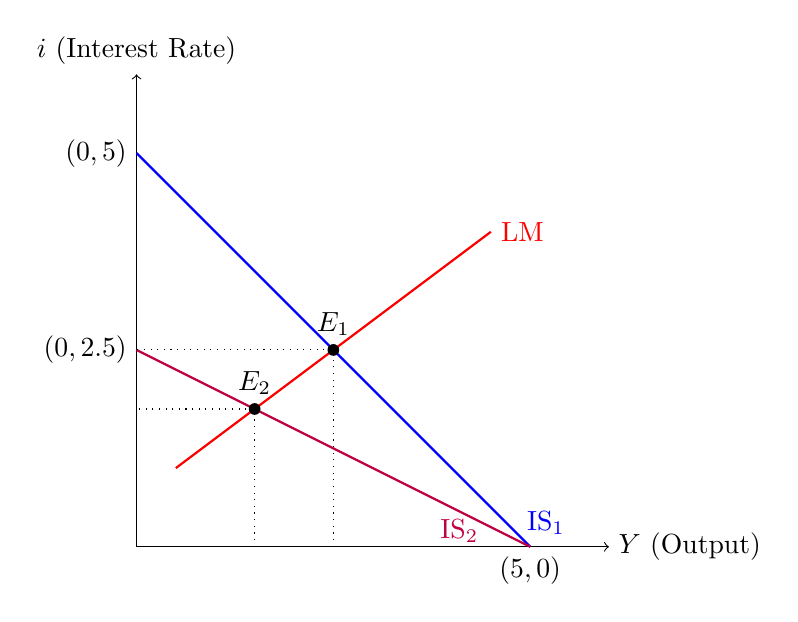
\begin{tikzpicture}[scale=1.0]
        \draw[->] (0,0) -- (6,0) node[right] {$Y$ (Output)};
        \draw[->] (0,0) -- (0,6) node[above] {$i$ (Interest Rate)};
        \draw[thick,blue] (0,5) -- (5,0) node[xshift=0.2cm, yshift=0.3cm] {$\text{IS}_1$};
        \node[left] at (0,5) {$(0,5)$};
        \node[below] at (5,0) {$(5,0)$};
        \draw[thick,purple] (0,2.5) -- (5,0) node[xshift=-0.9cm,yshift=0.2cm] {$\text{IS}_2$};
        \node[left] at (0,2.5) {$(0,2.5)$};
        \draw[thick,red] (0.5,1) -- (4.5,4) node[right] {LM};
        \draw[dotted] (2.5,0) -- (2.5,2.5) -- (0,2.5);
        \draw (2.5,2.5) node[circle,fill,inner sep=1.5pt]{};
        \node[yshift=0.33cm] at (2.5,2.5) {$E_1$};
        \draw[dotted] (1.5,0) -- (1.5,1.75) -- (0,1.75);
        \draw (1.5,1.75) node[circle,fill,inner sep=1.5pt]{};
        \node[yshift=0.33cm] at (1.5,1.75) {$E_2$};
    \end{tikzpicture}
    \caption{Both IS curves intersect at $(5,0)$, but $\text{IS}_2$ has a flatter slope 
    and intersects the vertical axis at $(0,2.5)$. 
    With an upward-sloping LM, the equilibrium shifts from $E_1$ to $E_2$, 
    showing lower output (leftward shift).}
\end{figure}
\noindent
\textbf{Interpretation:}
\begin{itemize}
    \item \(\text{IS}_1\) (\(i = 5 - Y\)) is steeper, meeting the axes at \((0,5)\) and \((5,0)\).
    \item \(\text{IS}_2\) (\(i = 2.5 - 0.5\,Y\)) is “flatter,” also crossing \((5,0)\) but hitting \((0,2.5)\) on the vertical axis.
    \item For any given interest rate \(i < 5\), the new IS curve implies a lower output \(Y\). This captures a “leftward shift” in equilibrium if the LM curve is upward sloping.
    \item \textbf{Why a leftward shift?} Because at typical policy rates below 5\%, investment is now more sensitive to risk premia, effectively reducing aggregate demand for the same safe interest rate.
\end{itemize}
\noindent
\textbf{Factors that Could Produce This Shift/Rotation:}
\begin{itemize}
    \item \emph{Higher Risk Premiums} (banks charge more when policy rates rise).
    \item \emph{Stricter Lending Standards} (reducing investment at any given policy rate).
    \item \emph{Regulatory Changes} that increase banks’ cost of lending, passed on to borrowers.
    \item \emph{Increased Uncertainty} or \emph{Worse Credit Quality} among firms and households.
\end{itemize}
\chapter*{The AD--AS Model}
\section*{Overview}
To make our analysis more realistic and to introduce inflation into the picture, we now present the AD--AS model in \((Y,\pi)\)-space. Here, the horizontal axis represents real output \(Y\) and the vertical axis represents inflation \(\pi\). In our model:
\begin{itemize}
    \item The \textbf{Aggregate Demand (AD)} curve is downward sloping. A higher inflation rate tends to reduce real balances and dampen consumption and investment, thereby lowering output.
    \item The \textbf{Short-Run Aggregate Supply (SAS)} curve is upward sloping. Due to nominal rigidities—such as sticky wages—higher inflation is associated with higher output in the short run.
    \item The \textbf{Classical Aggregate Supply (AS)} curve is vertical. It represents the economy's potential output \(Y^*\), which is determined by real factors like technology and resources. In the long run, inflation does not affect real output.
\end{itemize}
The figure below shows a typical AD--AS diagram with these characteristics. In this example, we set the potential output at \(Y^*=5\) and assume an equilibrium at \(E=(5,3)\).
\begin{figure}[ht]
    \centering
    \begin{tikzpicture}[scale=1.0]
        \draw[->] (0,0) -- (10,0) node[right] {\(Y\) (Output)};
        \draw[->] (0,0) -- (0,7) node[above] {\(\pi\) (Inflation)};
        \draw[thick] (5,0) -- (5,7) node[above left] {AS};
        \draw[thick,red] (1,1) -- (9,5) node[right] {SAS};
        \draw[thick,blue] (1,5) -- (9,1) node[right] {AD};
        \draw[dotted] (5,0) -- (5,3) -- (0,3);
        \fill (5,3) circle (2pt);
        \node[xshift=0.25cm, yshift=0.4cm] at (5,3) {\(E\)};
    \end{tikzpicture}
    \caption{AD--AS diagram in \((Y,\pi)\)-space. The downward-sloping AD (blue) and upward-sloping SAS (red) curves intersect at \(E=(5,3)\). The vertical AS curve (black) shows potential output \(Y^*=5\).}
\end{figure}

\bigskip

\noindent \textbf{Discussion:}
\begin{itemize}
    \item In the short run, if an aggregate demand shock occurs (e.g., expansionary fiscal policy), the AD curve shifts. Depending on the monetary policy response, the Central Bank may allow inflation to change.
    \item If the economy is operating below potential, downward pressure on wages may shift SAS rightward, eventually restoring equilibrium at the potential output (AS).
    \item The Taylor rule and the Central Bank's reaction function (adjusting interest rates to target a specific inflation rate) help determine the slope of the AD curve.
\end{itemize}

\section*{AD--AS Equilibrium and the Impact of Shocks}
\subsection*{Baseline Equilibrium}
In the long-run equilibrium the economy's actual output equals its potential output. For example, consider the following baseline curves in \((Y,\pi)\)-space:
\begin{itemize}
    \item \(\textbf{AD:}\) \(\pi = -0.5\,Y + 5.5\)
    \item \(\textbf{SAS:}\) \(\pi = 0.5\,Y + 0.5\)
    \item \(\textbf{AS:}\) Vertical line at \(Y^*=5\)
\end{itemize}
These curves intersect at the equilibrium point \(E_0=(5,3)\).
\begin{figure}[ht]
    \centering
    \begin{tikzpicture}[scale=1.0]
        \draw[->] (0,0) -- (10,0) node[right] {\(Y\) (Output)};
        \draw[->] (0,0) -- (0,7) node[above] {\(\pi\) (Inflation)};
        \draw[thick] (5,0) -- (5,7) node[above left] {AS};
        \draw[thick,red] (1,1) -- (9,5) node[right] {SAS};
        \draw[thick,blue] (1,5) -- (9,1) node[right] {AD};
        \draw[dotted] (5,0) -- (5,3) -- (0,3);
        \fill (5,3) circle (2pt);
        \node[xshift=0.25cm, yshift=0.4cm] at (5,3) {\(E_0\)};
    \end{tikzpicture}
    \caption{Baseline AD--AS diagram in \((Y,\pi)\)-space with \(E_0=(5,3)\) and potential output \(Y^*=5\).}
\end{figure}

\subsection*{Analysis of Shocks:}
Suppose the economy is hit by a severe shock---such as a major natural disaster---that:
\begin{itemize}
    \item \textbf{Negatively affects aggregate supply (AS):} The destruction of capital assets reduces production possibilities. Although some capital can be rebuilt over several years, adverse demographic impacts (e.g., loss of human capital) may make part of this shock permanent. Graphically, this shifts the short‑run aggregate supply (SAS) curve upward (reflecting higher production costs) and the classical aggregate supply (AS) curve leftward (reflecting a lower potential output).
    \item \textbf{Negatively affects aggregate demand (AD):} Losses in income and consumer confidence may also reduce spending. However, some types of spending may simply be re‐allocated (for example, from discretionary spending to rebuilding), so the AD shock may be more modest.
\end{itemize}
Below is a diagram illustrating a new, post-shock equilibrium. In our example, we assume:
\begin{itemize}
    \item The new potential output falls from \(Y^*=5\) to \(Y^*=4.5\) (AS shifts left).
    \item The SAS curve shifts upward by 1 unit (reflecting cost-push effects), so that the new SAS is given by: 
    \[
    \pi = 0.5\,Y + 1.5.
    \]
    \item The AD curve shifts left modestly, to, for example: 
    \[
    \pi = -0.5\,Y + 5.3.
    \]
\end{itemize}
The new short-run equilibrium \(E'\) is determined by the intersection of the new SAS and AD curves. Solving
\[
0.5\,Y + 1.5 = -0.5\,Y + 5.3,
\]
we find:
\[
Y = 3.8 \quad \text{and} \quad \pi = 0.5(3.8) + 1.5 \approx 3.4.
\]
Thus, \(E'=(3.8,3.4)\).
\begin{figure}[ht]
    \centering
    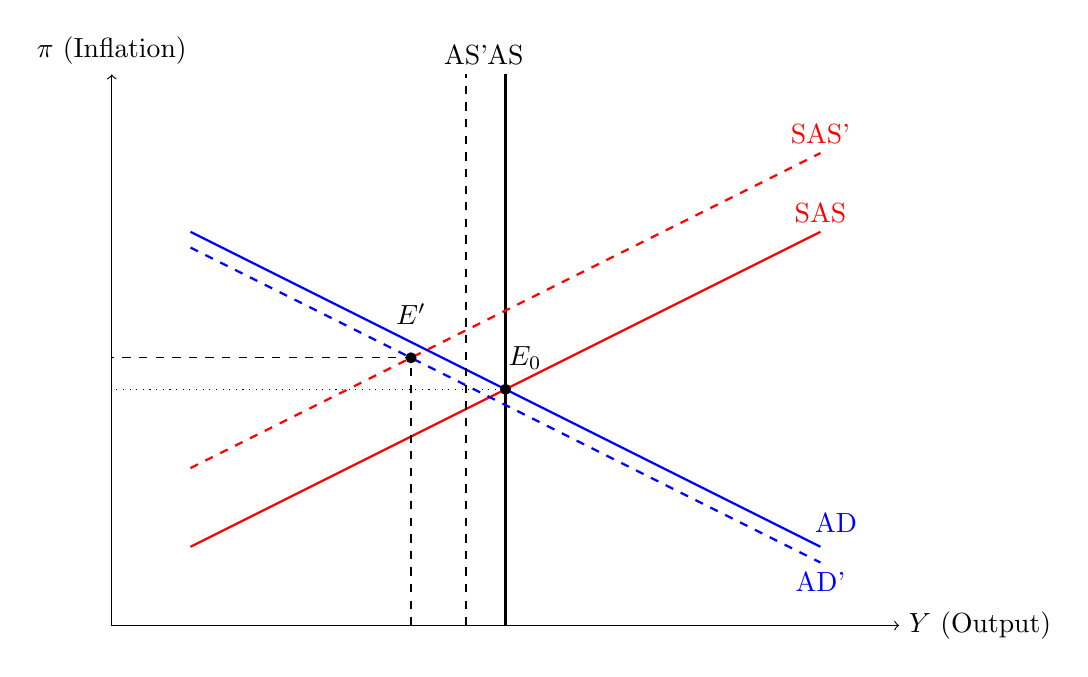
\begin{tikzpicture}[scale=1.0]
        \draw[->] (0,0) -- (10,0) node[right] {\(Y\) (Output)};
        \draw[->] (0,0) -- (0,7) node[above] {\(\pi\) (Inflation)};
        \draw[thick] (5,0) -- (5,7);
        \node[above] at (5,7) {AS};
        \draw[thick,red] (1,1) -- (9,5);
        \node[red,above] at (9,5) {SAS};
        \draw[thick,blue] (1,5) -- (9,1);
        \node[blue,xshift=0.2cm, yshift=0.3cm] at (9,1) {AD};
        \draw[dotted] (5,0) -- (5,3) -- (0,3);
        \fill (5,3) circle (2pt);
        \node[xshift=0.25cm, yshift=0.4cm] at (5,3) {\(E_0\)};
        \draw[thick,dashed] (4.5,0) -- (4.5,7);
        \node[above] at (4.5,7) {AS'};
        \draw[thick,red,dashed] (1,2) -- (9,6);
        \node[red,above] at (9,6) {SAS'};
        \draw[thick,blue,dashed] (1,4.8) -- (9,0.8);
        \node[blue,below] at (9,0.8) {AD'};
        \draw[dotted,dashed] (3.8,0) -- (3.8,3.4) -- (0,3.4);
        \fill (3.8,3.4) circle (2pt);
        \node[above=0.3cm] at (3.8,3.4) {\(E'\)};
    \end{tikzpicture}
    \caption{Updated AD--AS diagram with dashed post-shock curves and non-overlapping labels. 
    Baseline curves (solid) intersect at \(E_0\); new curves (dashed) intersect at \(E'\).}
\end{figure}

\subsection*{Interpretation of the Shocks}
\begin{itemize}
    \item \textbf{Aggregate Supply Shock:}  
    The disaster reduces the economy’s production capacity. The short-run aggregate supply (SAS) curve shifts upward due to higher costs, while the long-run (classical) aggregate supply (AS) shifts left, indicating a lower potential output. Although some capital can be rebuilt over time, adverse demographic effects mean that a portion of the shock is permanent.
    \item \textbf{Aggregate Demand Shock:}  
    The loss of income and confidence tends to reduce consumption and investment, shifting the aggregate demand (AD) curve leftward. However, some planned spending may simply be redirected (for example, from leisure to reconstruction), so the demand shock may be relatively modest.
    \item \textbf{New Equilibrium:}  
    The combined effects of the shocks result in a new short-run equilibrium \(E'\) with lower output and a slightly higher inflation rate. In this example, output falls from 5 to about 3.8 and inflation rises from 3 to 3.4, illustrating how negative supply shocks (with some permanent components) can lead to stagflation.
\end{itemize}
\chapter*{Macro Lecture II.1: Introduction to Macroeconomics, GDP, and the Circular Flow Model}
\section*{Overview}
This lecture introduces macroeconomics at the aggregate level, focusing on the measurement of national output and income through GDP, and explains the circular flow model that illustrates the interactions among households, firms, government, and the foreign sector.

\section*{Key Concepts in Macroeconomics}
\begin{itemize}
    \item \textbf{Aggregate Analysis:} Examines the economy as a whole rather than individual markets.
    \item \textbf{General Equilibrium:} Considers the simultaneous equilibrium in goods, factor, and financial markets.
    \item \textbf{Core Issues:} Economic growth, inflation, unemployment, business cycles, and economic crises.
\end{itemize}

\section*{GDP and National Income Statistics}
\begin{itemize}
    \item \textbf{Definition of GDP:} The market value of final goods and services produced within a country over a given period.
    \item \textbf{Methods of Computing GDP:}
    \begin{itemize}
        \item \textbf{Output (Value Added) Approach:} Summing the value added at each stage of production.
        \item \textbf{Expenditure Approach:} Adding up consumption (C), investment (I), government spending (G), and net exports (exports $X$ minus imports $Z$):
        \[
        GDP = C + I + G + (X - Z)
        \]
        \item \textbf{Income Approach:} Summing incomes earned by households and firms (wages, profits, etc.).
    \end{itemize}
    \item \textbf{Nominal vs. Real GDP:}
    \begin{itemize}
        \item \textbf{Nominal GDP:} Calculated at current market prices.
        \item \textbf{Real GDP:} Calculated at constant prices to adjust for inflation.
    \end{itemize}
    \item \textbf{GDP Deflator:} A measure of the price level, defined as the ratio of Nominal GDP to Real GDP.
\end{itemize}

\section*{The Circular Flow Model}
\begin{itemize}
    \item \textbf{Basic Framework:} Describes how money flows between households and firms through the exchange of goods, services, and factors of production.
    \item \textbf{Leakages and Injections:}
    \begin{itemize}
        \item \textbf{Leakages:} Portions of income not spent on domestic goods and services, such as savings, taxes, and imports.
        \item \textbf{Injections:} Additional spending into the economy, such as investment, government spending, and exports.
    \end{itemize}
    \item \textbf{Savings and Investment Identity:}
    \[
    Y = C + S \quad \text{and} \quad Y = C + I \quad \Rightarrow \quad S = I
    \]
    \item \textbf{Role of Government and Foreign Sector:} Government activities (taxes and spending) and foreign trade (exports and imports) further modify the flow of income.
\end{itemize}

\section*{Additional Discussion Points}
\begin{itemize}
    \item The importance of using market values and focusing on final goods to avoid double counting.
    \item How GDP per capita is used as an indicator of average living standards.
    \item The implications of including unsold inventory as investment in GDP.
\end{itemize}
\chapter*{Macro Lecture II.2: Output and Aggregate Demand -- The Keynesian Cross Model}
\section*{Overview}
This lecture presents the basic short-run goods-and-services market model, emphasizing the Keynesian cross framework. It covers equilibrium in the goods market, the multiplier effect, the paradox of thrift, and the role of government in aggregate demand.

\section*{The Basic Model without Government}
\begin{itemize}
    \item \textbf{Consumption Function:}
    \[
    C = A + cY
    \]
    where \(A\) is autonomous consumption and \(c\) (with \(0 < c < 1\)) is the marginal propensity to consume (MPC).
    \item \textbf{Investment:}
    \[
    I = \bar{I}
    \]
    (investment is treated as exogenous).
    \item \textbf{Aggregate Demand (AD):}
    \[
    AD = A + cY + \bar{I}
    \]
    \item \textbf{Equilibrium Condition:}
    \[
    Y = AD = A + cY + \bar{I}
    \]
    Solving for equilibrium output:
    \[
    Y^* = \frac{A + \bar{I}}{1 - c}
    \]
    Here, \(\frac{1}{1-c}\) is the multiplier.
\end{itemize}

\section*{Market Adjustments and Disequilibria}
\begin{itemize}
    \item When actual output \(Y\) is below \(Y^*\), aggregate demand exceeds output, leading to unplanned reductions in inventories and signaling firms to increase production.
    \item Conversely, when \(Y\) exceeds \(Y^*\), firms face unsold inventories, prompting a reduction in output.
\end{itemize}

\section*{Investment Equals Saving}
In equilibrium, the goods market satisfies:
\[
Y = C + I \quad \Rightarrow \quad S = Y - C = I
\]

\section*{Extension: Adding Government}
\begin{itemize}
    \item With government, disposable income is:
    \[
    Y_d = (1-t)Y
    \]
    where \(t\) is the net tax rate.
    \item The consumption function becomes:
    \[
    C = A + c(1-t)Y
    \]
    \item The equilibrium condition now is:
    \[
    Y = A + c(1-t)Y + \bar{I} + G
    \]
    Solving for \(Y^*\):
    \[
    Y^* = \frac{A + \bar{I} + G}{1 - c(1-t)}
    \]
\end{itemize}

\section*{Balanced Budget Multiplier}
\begin{itemize}
    \item If government spending \(G\) increases by 1 dollar and is financed by an equal increase in taxes, the equilibrium output will increase. Under certain conditions, the balanced budget multiplier is equal to 1.
\end{itemize}

\section*{Additional Discussion}
\begin{itemize}
    \item \textbf{Actual vs. Potential Output:} While potential output is fixed in the short run, actual output can deviate, leading to economic recessions or expansions.
    \item \textbf{Paradox of Thrift:} An increase in household savings (modeled as a decrease in \(A\)) may reduce aggregate demand and lower equilibrium output, leaving overall private saving unchanged but reducing total income.
\end{itemize}
\chapter*{Macro Lecture II.3: The Keynesian Cross Model, Part 2 -- Money and Banking}
\section*{Overview}
This lecture extends the Keynesian cross framework by incorporating topics on fiscal policy, the foreign sector, and, in depth, money and banking. It discusses how monetary policy and banking operations interact with aggregate demand and influence the economy.

\section*{Fiscal Policy, Budget, and the Foreign Sector}
\begin{itemize}
    \item \textbf{Fiscal Policy and Fiscal Stance:} 
    \begin{itemize}
        \item Fiscal policy is the government’s use of spending and taxation to influence aggregate demand.
        \item The \emph{fiscal stance} indicates whether the policy is expansionary (budget deficit) or contractionary (budget surplus).
        \item Adjustments such as structural budgets and inflation-adjusted budgets are used to assess the true fiscal stance.
    \end{itemize}
    \item \textbf{Budget Deficit and Debt:}
    \begin{itemize}
        \item Governments often finance deficits via debt. A key indicator is the debt-to-GDP ratio.
        \item Strategies for coping with debt include promoting nominal GDP growth, using inflation to reduce real debt burdens, or, in extreme cases, default.
    \end{itemize}
    \item \textbf{Adding the Foreign Sector:}
    \begin{itemize}
        \item Net exports (NX) are defined as \(NX = X - Z\), where exports \(X\) are typically treated as exogenous and imports \(Z\) are modeled as \(Z = zY\).
        \item The equilibrium condition is then extended to:
        \[
        Y = C + I + G + X - zY
        \]
    \end{itemize}
\end{itemize}

\section*{Money and Banking}
\begin{itemize}
    \item \textbf{Definitions and Money Aggregates:}
    \begin{itemize}
        \item \emph{M0} is the currency outside banks.
        \item \emph{MB} (monetary base) equals cash plus bank reserves.
        \item \emph{M1} includes cash and demand deposits.
    \end{itemize}
    \item \textbf{Banking Operations and Money Creation:}
    \begin{itemize}
        \item A commercial bank’s balance sheet satisfies:
        \[
        \text{Assets} = \text{Liabilities} + \text{Equity}
        \]
        \item Money creation occurs through the deposit and loan multipliers:
        \[
        \text{Deposit Multiplier} = \frac{1}{rr}, \quad \text{Loan Multiplier} = \frac{1 - rr}{rr}
        \]
    \end{itemize}
    \item \textbf{Money Multiplier:}
    \[
    mm = \frac{1 + cr}{cr + rr + er}
    \]
    where the ratios \(cr\), \(rr\), and \(er\) capture public preferences and banking regulations.
    \item \textbf{Money Market Equilibrium:}
    \begin{itemize}
        \item Equilibrium in the money market is reached when money demand \(M_d(Y, r)\) equals money supply \(M_s\).
        \item Real money balances are expressed as \(\frac{M}{P}\).
    \end{itemize}
\end{itemize}

\section*{Monetary Policy and Its Instruments}
\begin{itemize}
    \item \textbf{Objectives:} The Central Bank conducts monetary policy to stabilize output and promote economic growth.
    \item \textbf{Instruments:}
    \begin{itemize}
        \item \emph{Required Reserve Ratio:} Adjusting this influences the amount of money banks can create.
        \item \emph{Open Market Operations:} Buying or selling government bonds to change the monetary base.
        \item \emph{Discount Rate:} Changing the rate at which commercial banks borrow from the Central Bank affects bank reserves and lending.
    \end{itemize}
    \item \textbf{Transmission Mechanism:}
    \begin{itemize}
        \item Lower interest rates stimulate investment and consumption.
        \item The overall effect of monetary policy is transmitted through changes in aggregate demand.
    \end{itemize}
\end{itemize}
\chapter*{Macro Lecture II.4: Fiscal and Monetary Policy -- The IS-MP (IS-LM) Model}
\section*{Overview}
This lecture integrates fiscal and monetary policy into the general equilibrium framework of the goods and money markets using the IS-MP (IS-LM) model. With fixed prices, the model explains how output and interest rates are jointly determined by both fiscal actions and monetary policy.

\section*{The IS Curve: Goods Market Equilibrium}
\begin{itemize}
    \item \textbf{Goods Market Equilibrium:} The equilibrium condition is given by
    \[
    Y = C + I + G + NX.
    \]
    \item \textbf{Modified Consumption and Investment Functions:}
    \begin{itemize}
        \item Consumption: 
        \[
        C = A_0 - a \cdot i + c(1-t)Y.
        \]
        \item Investment:
        \[
        I = I_0 + \text{mpi} \cdot Y - b \cdot i.
        \]
    \end{itemize}
    \item \textbf{Derivation of the IS Curve:} Combining the above functions, the equilibrium condition becomes:
    \[
    Y\Bigl(1 - c(1-t) - \text{mpi} + z\Bigr) = \Bigl[A_0 + I_0 + G + X\Bigr] - (a+b)i,
    \]
    which can be rearranged to express output \(Y\) as a function of the interest rate \(i\).
\end{itemize}

\section*{The MP Curve: Monetary Policy Rule}
\begin{itemize}
    \item The MP curve represents combinations of output \(Y\) and the interest rate \(i\) that satisfy money market equilibrium.
    \item Under the fixed price assumption, nominal and real interest rates coincide.
    \item The Central Bank adjusts \(i\) to stabilize output---lowering \(i\) when output is below potential and raising \(i\) when output exceeds potential.
\end{itemize}

\section*{General Equilibrium and Policy Analysis}
\begin{itemize}
    \item \textbf{Equilibrium:} General equilibrium is achieved where the IS and MP curves intersect, determining the equilibrium output \(Y^*\) and interest rate \(i^*\).
    \item \textbf{Policy Implications:}
    \begin{itemize}
        \item \emph{Fiscal Policy:} Changes in government spending \(G\) or taxation \(T\) shift the IS curve.
        \item \emph{Monetary Policy:} Adjustments to the interest rate target shift the MP curve.
        \item \emph{Crowding Out:} The degree to which government spending crowds out private investment depends on the slopes of the IS and MP curves.
    \end{itemize}
    \item \textbf{Analysis Steps:}
    \begin{enumerate}
        \item Identify shifts in the IS and/or MP curves.
        \item Determine the new equilibrium \((Y^*, i^*)\).
        \item Discuss the resulting effects on both the goods and money markets.
    \end{enumerate}
\end{itemize}
\chapter*{Macro Lecture II.5: The AD-AS Model}
\section*{Overview}
This lecture introduces the AD-AS framework, which integrates the goods, money, and labor markets to analyze how aggregate demand and aggregate supply determine both output and the price level. The model accommodates adjustments to shocks in both AD and AS.

\section*{Aggregate Demand (AD)}
\begin{itemize}
    \item AD is the total spending on final goods and services and is given by:
    \[
    AD = C + I + G + (X - Z)
    \]
    \item Monetary policy influences AD through its impact on consumption and investment.
    \item Higher inflation typically leads the Central Bank to raise real interest rates, reducing consumption and investment, thereby shifting AD leftward.
\end{itemize}

\section*{Aggregate Supply (AS)}
\begin{itemize}
    \item \textbf{Long-Run Aggregate Supply (LRAS):} With fully flexible wages and prices, the economy produces at its potential output:
    \[
    Y = Y^*
    \]
    \begin{itemize}
        \item \textbf{Potential Output:} Defined as the level of output achieved when every market in the economy is in long-run equilibrium and all economic agents correctly anticipate economic conditions. It represents the sustainable level of production, not the maximum possible output.
    \end{itemize}
    \item \textbf{Short-Run Aggregate Supply (SRAS):} Due to sticky wages, SRAS is upward sloping. Firms adjust production based on the real wage:
    \[
    MP_L = \frac{w}{p}
    \]
    \item \textbf{Shifts in SRAS:}
    \begin{itemize}
        \item When output is below potential, higher unemployment may lead to lower nominal wages, shifting SRAS rightward.
        \item When output exceeds potential, rising wage demands shift SRAS leftward.
    \end{itemize}
\end{itemize}

\section*{Adjustment Mechanisms}
\begin{itemize}
    \item \textbf{AD Shocks:} Changes in fiscal or monetary policy can shift AD. The Central Bank may adjust interest rates to counteract inflationary or deflationary pressures.
    \item \textbf{AS Shocks:} Temporary supply shocks affect SRAS without altering potential output, whereas permanent shocks can shift both SRAS and LRAS.
\end{itemize}

\section*{The Taylor Rule and Monetary Policy}
\begin{itemize}
    \item The Taylor rule guides Central Bank policy by adjusting the nominal interest rate based on deviations of inflation and output from their targets:
    \[
    i - i^* = (1+a)(\pi - \pi^*) + b(Y - Y^*)
    \]
    \item This rule helps stabilize inflation while influencing aggregate demand.
\end{itemize}

\end{document}

\end{document}